% !Mode:: "TeX:UTF-8"
% !TEX program  = xelatex

%\documentclass{cumcmthesis}
\documentclass[withoutpre]{cumcmthesis} %去掉封面与编号页
\usepackage[framemethod=TikZ]{mdframed}
\usepackage{url}   % 网页链接
\usepackage{subcaption} % 子标题
\title{基于修正SEIR模型的新冠肺炎疫情预测与评估}
\tihao{A}
\baominghao{202010038016}
\schoolname{南京大学}
\membera{陈万驰 181840033 数学系}
\memberb{姜玉骅 181870080 工程管理学院}
\memberc{佘帅杰 181860077 计算机科学与技术系}
\supervisor{教练组}
\yearinput{2020}
\monthinput{08}
\dayinput{1}

\begin{document}

 \maketitle
 \begin{abstract}
    2020 年伊始,随着新型冠状病毒感染肺炎的迅速蔓延,全国笼罩在了疫
    情的阴影下,一时间几乎整个中国只有一个主题,就是如何共同抗击新型冠
    状病毒疫情(以下简称新冠疫情)。本文结合基于新冠病毒特征修改的SEIR
    传染病模型,对武汉市的疫情发展进行了模拟和对防控措施进行了评估,以
    及对印度疫情发展进行了模拟和预测。比较了单次检测和混样检测方法,给
    出了已知病毒携带率的条件下可以采取的检测次数最少的方案。

    针对问题一,基于传染病状况以及武汉市政府采取的控制措施,我们建
    立了一个修正的SEIR 模型,将人群分为易感者$(S)$、潜伏者$(E)$、感染者
    $(I)$、住院者$(H)$、移出者$(R)$、被隔离易感者$(S_q)$、被隔离潜伏者者$(E_q)$。
    在通过查阅参考文献以及经过适当调试之后,我们确定了各种人群之间相
    互转化的比率并建立了微分方程来表示转化过程。对微分方程求解之后我
    们得到了对武汉疫情发展的预测图像并将之与实际情况比对,最终我们得
    到了比较符合武汉实际情况的预测数据。

    针对问题二,基于问题一所建立的模型,我们通过改变隔离率、接触率、
    治愈率的取值来模拟不同严格程度的隔离措施对疫情发展的影响。通过观
    察数据及图像,发现武汉诸多严格的措施对疫情防控产生了巨大的正面影
    响。这也说明了在我国疫情防控初期,全国医护人员支援武汉的必要性和其
    积极影响。

    针对问题三,我们选取印度共和国作为此题的研究对象。印度是世界第
    二人口大国,庞大的人口基数和较不均衡的发展使得该国在疫情防控方面面
    临巨大的压力。通过对问题一建立的模型进行适当的修改和调试,利用官方
    发布的感染数据,我们绘制出了印度疫情发展的相关图像。通过观察预测数
    据和图像,我们发现如果不加强防控措施,印度的疫情还将呈指数型增长。

    针对问题四,我们利用伯努利分布对混样检测方式进行建模,
    将单人所需检测次数的期望作为优化的目标函数。在给定病毒携带者
    比例的条件下,我们利用下降单纯形法(Downhill Simplex)算出了使得目
    标函数最小的混样检测样本数量。最终,我们绘制了目标函数最小值与人群病毒携带率的关系图像并得出结论:在预期病毒携带者大于30\% 的地区,应该采取单人检测的方法,在小于30\% 的地方,应该采取混样检测的方法。

\keywords{新冠肺炎疫情 \quad SEIR 模型 \quad 混样检测}
\end{abstract}

%目录  2019 明确不要目录,我觉得这个规定太好了
%\tableofcontents

%\newpage

\section{问题背景与重述}
2019年12月初,武汉爆发新型冠状病毒(COVID-19)疫情,很快蔓延到全国各地,并在世界各国大流行。时至当下,病毒仍然在世界许多国家肆虐,世界各国人民的正常生活、生命健康以及社会经济持续受到威胁。由此,对新型冠状病毒的传播建立数学模型就非常有意义。

题目要求解决以下四个问题:
\begin{enumerate}
    \item 根据国家卫生健康委员会每日疫情通报数据,建立武汉市新型冠状病毒传播数学模型(需给出2月12日由于确诊标准改变而产生数据突变的合理方案),评价其合理性和实用性。
    \item 说明2020年1月23号武汉封城、2020年1月下旬武汉新建雷神山医院和火神山医院、2月初建立了20家方舱医院、武汉市市民居家隔离、全国各地有近4.2万医务人员驰援武汉抗击疫情等一系列措施在控制疫情发展中发挥的作用,如果没有采取(或提早、延后采取),对疫情传播所产生的影响作出评估。
    \item 根据世界卫生组织报告的疫情通报,选定某个国家和地区疫情数据,建立数学模型,评价其合理性和实用性
    \item 给出面对给定人群中预期病毒携带者的比例,采用单次检测还是混样检测(混检分组方式),达到既可以筛选病毒携带者,同时检测次数最少的方案。
\end{enumerate}

\section{问题分析}
\subsection{问题一分析}
疫情传播类问题,可将人群分为易感者(Susceptible,$S$)、感染者(Infected,$I$)、潜伏者(Exposed,$E$)和移除人群(Removed,$R$),即经典的SEIR模型。考虑到新冠肺炎的隔离措施,在SEIR模型的基础上添加隔离人群以适用实际情况。由于各个时间段疫情防护的严格程度不同,建立模型选取的参数不能一概而论,因此可以考虑划分时间段,不同时间段选取不同的模型参数。如果以2月12日作为一个时间段分割点,这也能解决2月12日由于确诊标准改变而产生数据突变的拟合问题。

\subsection{问题二分析}
各种防护措施影响的是模型参数的选取,如接触率、感染率、治愈率等。通过分析措施对参数的影响,将参数的变化映射到模型的变化,即能评估出该措施对疫情传播产生的影响。

\subsection{问题三分析}
问题三与问题一基本一致,考虑沿用问题一的模型,用于建立印度新冠肺炎疫情传播模型,对疫情发展进行了模拟和预测。

\subsection{问题四分析}
欲比较混样检测和单次检测方法,单次检测方法即每人检测次数为一次,因此问题转变为给定人群病毒携带率,混样检测平均每人检测次数是否少于1。若是则考虑使用混样检测方法,否则使用单次检测方法。

混样检测,顾名思义就是将几个样本混合在一起进行一次核酸检测。某次需要对$N$个人进行检测,病毒的携带率为$p$。为了减少工作量,一次性将$k$个人的样本混合,如果混合样本为阴性,则说明这$k$个人都没有患病。如果混合样本为阳性,说明这$k$个人中至少有1个人的样本是阳性,那么接下来对这$k$个人的分别单独做检测。而单次检测简单直观,即对所有人单独做检测。考虑用基本概率论知识,比较混样检测和单次检测方法对应到平均每人的检测次数,选取更合理的方案。

\section{模型假设}
\begin{enumerate}
    \item 假设人群中所有个体都有被感染的概率。
    \item 假设被感染个体痊愈后,会产生抗体,不会再被感染。
    \item 假设所有感染者是同质的,即病情的严重程度、死亡率相同。
    \item 鉴于1月23日武汉市封城,假设武汉市总人口的不变。
    \item 假设核酸检测准确率为100\%。
    \item 假设混样检测的结果不会因混样而改变,即若至少有一人感染,混样检测呈阳性;若无人感染,混样检测呈阴性。
\end{enumerate}

\section{符号说明}
\begin{table}[H]
    \caption{符号说明表}\label{tab:001} \centering
    \begin{tabular}{ccc}
        \toprule[1.5pt]
        \textbf{参数} & \textbf{定义} & \textbf{单位}\\
        \midrule[1pt]
        $W$ & 负重上限 & 千克\\ 
        $M$ & 初始资金 & 元 \\
        $t$ & 天数 & 天\\
        $T$ & 总天数 & 天\\
        $m_w$ & 每箱水的质量 & 千克/箱\\
        $m_f$ & 每箱食物的质量 & 千克/箱 \\
        $p_w$ & 水的基准价格 & 元/箱\\
        $p_f$ & 食物的基准价格 & 元/箱\\
        $n_{sw}$ & 晴朗天气下水的基准消耗量 & 箱\\
        $n_{hw}$ & 高温天气下水的基准消耗量 & 箱\\
        $n_{ow}$ & 沙暴天气下水的基准消耗量 & 箱\\
        $n_{sf}$ & 晴朗天气下食物的基准消耗量 & 箱\\
        $n_{hf}$ & 高温天气下食物的基准消耗量 & 箱\\
        $n_{of}$ & 沙暴天气下食物的基准消耗量 & 箱\\
        $n$ & 玩家数 & 人 \\
        $P_{it}$ & 第t天开始时玩家i所处的位置 & / \\
        $W_{it}$ & 第t天开始时玩家i剩余的水 & 箱 \\
        $F_{it}$ & 第t天开始时玩家i剩余的食物 & 箱 \\ 
        $Q_{it}$ & 第t天开始时玩家i剩余的资金 & 元 \\
        $We_t$ & 第t天的天气 & /\\
        $S_{it}$ & 第t天玩家i所处的地点特征 & /\\
        \bottomrule[1.5pt]
    \end{tabular}
\end{table}


\section{模型建立与分析}
\subsection{问题一}
基于传染病状况以及政府采取的控制措施,我们建立了一个修正的SEIR模型。将人群分为易感者($S$)、潜伏者($E$)、感染者($I$)、住院者($H$)、移除者($R$)、被隔离易感者($S_q$)、被隔离潜伏者者($E_q$)。住院者(H)即隔离的感染者,考虑到部分感染者由于病房不足等原因无法入院治疗,因此将住院者与感染者分开界限。$S$、$I$、$E$分别指未采取强制隔离措施的易感者、感染者和潜伏者。若人群总人数为N,则
\begin{equation}
    S + E + I + H + R + S_q + E_q = N
\end{equation}
用$q$表示隔离率,表示易感者若接触感染者被隔离的概率,隔离的易感者$S_q$隔离期间(隔离时长为$\frac{1}{\lambda}$)未发现异常将解除隔离回到$S$中。相对应,隔离的潜伏者$E_q$度过潜伏期后出现症状将转变为住院患者$H$。同样存在未被隔离的易感者也以一定概率转变为潜伏者,度过潜伏期成为感染者,以一定几率被隔离成为住院患者或者死亡或者被治愈。需要注意的是确诊者人数等于住院患者人数加感染者人数,移除者中包含死亡和治愈的人群。详细人群转化关系如\cref{fig:transmission}所示。
\begin{figure}[H]
    \centering
    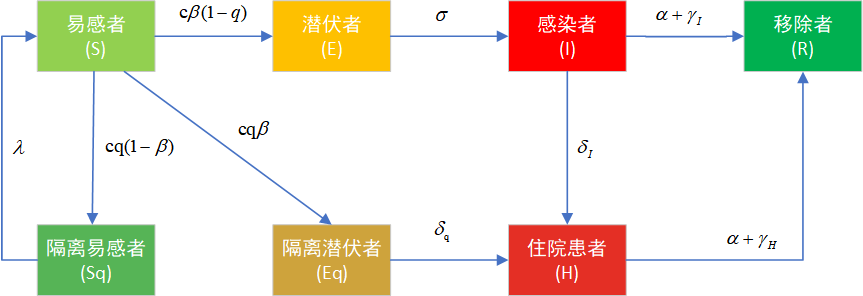
\includegraphics[width=\textwidth]{figures/transmission.png}
    \caption{人群转化关系图}
    \label{fig:transmission}
\end{figure}

其中$c$为接触率,$\beta$为传染概率,$\sigma$为潜伏者向感染者的转化速率,$\alpha$为病死率,$\delta_I$为感染者的隔离速率,$\gamma_I$是感染者的治愈率。$\delta_q$是隔离潜伏者向隔离感染者的转化速率,$\gamma_H$是住院患者(隔离感染者)的治愈率。

本文所用的修正SEIR模型中,各人群增长速率如下:
\begin{equation}
    \left\{\begin{array}{l}
        \displaystyle \frac{d S}{d t}=-[  c \beta+  c q(1-\beta)] S(I+\theta E)+\lambda S_{q} \\ \\
        \displaystyle \frac{dE}{dt}=  c \beta(1-q) S(I+\theta E)-\sigma E \\ \\
        \displaystyle \frac{dI}{dt}=\sigma E-\left(\delta_{I}+\alpha+\gamma_{I}\right) I \\ \\
        \displaystyle \frac{dS_q}{dt} =  c q(1-\beta) S(I+\theta E)-\lambda S_{q} \\ \\
        \displaystyle \frac{dE_q}{dt}=  c \beta q S(I+\theta E)-\delta_{q} E_{q} \\ \\
        \displaystyle\frac{dH}{dt}=\delta_{I} I+\delta_{q} E_{q}-\left(\alpha+\gamma_{H}\right) H \\ \\
        \displaystyle\frac{dR}{dt}=(\alpha + \gamma_{I})I+(\alpha + \gamma_{H})H
        \end{array}\right.
    \label{equation:1}
\end{equation}
给定所有参数值以及人群初值上述常微分方程组可以用Python 科学计算库Sicpy中的scipy.integrate.odeint()函数很方便的求解模型。但模型的求解难度在于如何设定参数值及人群初值。

 \cite{reference1}中采用数据处理、最小二乘法、MCMC方法确定模型未知参数, \cite{reference2}在 \cite{reference1}模型参数的基础上加以修正,提高了模型在整个湖北省疫情传播预测的准确度。本文借鉴上述文献的模型参数,求解武汉市1月23日到4月27日疫情转播模型。考虑到疫情阶段防护措施、医疗条件不断改变,并且2月12日确诊标准改变,模型参数如接触率$c$,隔离率$q$,治愈率$\gamma_H$随着时间的推移,理论上应该加以改变。因此本文将模型分为三个时间段:1月23日到2月11日、2月12日到2月21日、2月22日到4月27日,分别设定不同接触率$c$,隔离率$q$,治愈率$\gamma_H$求解模型。其余参数及模型初值参考了 \cite{reference1}、 \cite{reference2},并在各个时间段内保持一致,分别见\cref{tab:para},\cref{tab:value}。

\begin{table}[H]\small
    \caption{修正SEIR模型参数取值}
    \label{tab:para} \centering
    \begin{tabular}{p{1.5cm}p{2cm}p{1cm}p{1cm}p{1cm}p{2cm}p{1.5cm}p{1.5cm}p{1cm}}
        \toprule[1.5pt]
        \textbf{变量} & $\beta$ & $\delta_I$ & $\delta_H$ & $\gamma_I$ & $\alpha$ & $\sigma $ & $\lambda$ &$\theta$\\
        \midrule[1pt]
        \textbf{取值} & $2.05 \times 10^{-9}$ & 0.13& 0.13& 0.007& $ 2.7 \times 10^{-4} $ & 1/7& 1/14&1\\
        \textbf{取值说明} &  \cite{reference2}&  \cite{reference1}&  \cite{reference1}&  \cite{reference2}&  \cite{reference2}&潜伏期时长为7天 & 隔离时长为14天& \cite{reference2}\\
        \bottomrule[1.5pt]
    \end{tabular}
\end{table}

\begin{table}[H]\small
    \caption{修正SEIR模型人群初始值}
    \label{tab:value} \centering
    \begin{tabular}{p{1.5cm}p{2cm}p{3cm}p{1cm}p{1cm}p{1cm}p{1cm}p{1cm}}
        \toprule[1.5pt]
        \textbf{变量} & $S$ & $E$ & $I$ & $S_q$ & $E_q$ & $H$ & $R$  \\
        \midrule[1pt]
        \textbf{取值} & 1108100& 630& 410& 739& 20& 41&2 \\
        \textbf{取值说明} & 武汉市总人口数,参考 \cite{reference1}& 武汉1月29日确诊人数与1月23日确诊人数的差值&  \cite{reference1}&  \cite{reference1} &  \cite{reference1}& \cite{reference1} &  \cite{reference1}\\
        \bottomrule[1.5pt]
    \end{tabular}
\end{table}

接触率$c$、隔离率$q$、治愈率$\gamma_H$的取值根据三个阶段实际数据进行拟合优化,采用均方根误差的最小约束原则以及模拟退火的方法求解三个时间段模型最优解对应的参数值,结果见\cref{tab:optipara}

\begin{table}[H]
    \caption{修正SEIR模型三阶段参数优化值}
    \label{tab:optipara} \centering
    \begin{tabular}{p{5cm}p{3cm}p{3cm}p{3cm}}
        \toprule[1.5pt]
        \textbf{时间段} & $c$ & $q$ & $\gamma_H$ \\
        \midrule[1pt]
        1月23至2月11日 &12.5&  $4.37 \times 10^{-7}$& 0.014\\
        2月12日至2月21日& 11.7& $3.6\times 10^{-4}$&0.040 \\
        2月22日至4月27日 &0.37&1&0.080 \\
        \bottomrule[1.5pt]
    \end{tabular}
\end{table}

\cref{tab:optipara}中三个时间段,随着时间的推移,接触率$c$依次降低、隔离率$q$依次增加、住院患者治愈率$\gamma_H$依次增加。反映了随着疫情的发展,防护措施逐渐得当、医疗水平不断提升。早期的接触率达到2位数,末期的接触率变为小数,也能充分反映了武汉市疫情前后,个人防护意识、政府防护措施的严格有效。 

武汉疫情传播模型求解结果如\cref{fig:model}。
\begin{figure}[!h]
    \centering
    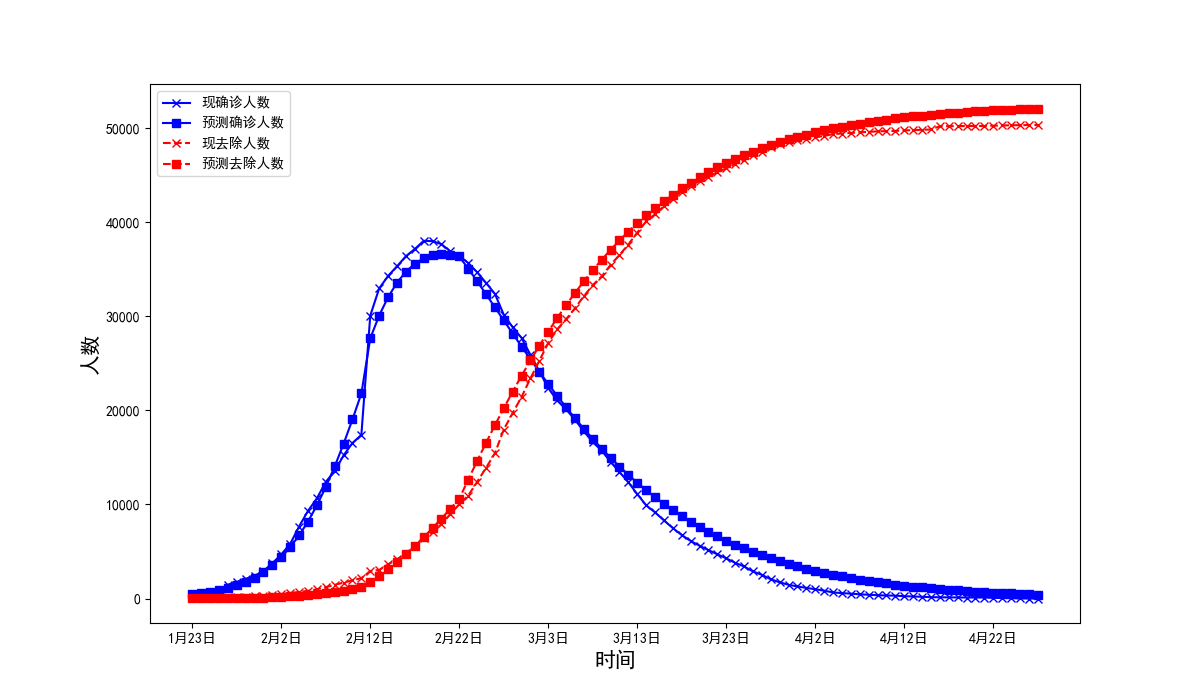
\includegraphics[width=1.0\textwidth]{figures/Model_predict_and_realNum_Graph.png}
    \caption{修正的SEIR模型对武汉市疫情的传播预测}
    \label{fig:model}
\end{figure}

分析发现,基于本文建立的修正SEIR模型估计的武汉市确诊(感染者+住院患者)人数在2020年1月23日到2020年2月8日、以及2020年2月22日到2020年4月27日时间段内与实际确诊人数吻合较好,去除人数(死亡+治愈)与实际去除人数全程吻合较好。美中不足的地方在于2月9日至2月21日时间段,由于2月12日确诊标准变化导致的数据突变,预测与实际存在些许偏差。可以解释的是,2月12日确诊标准的改变导致2月12日附近时间段内,实际的确诊人数与真实人群中的确诊人数有所误差,本文建立的模型相当于平滑了2月12日的数据突变,较均匀的将确诊人数分布到附近时间段,实际上更吻合真实环境中确诊者人数的变化。

\subsection{问题二}
2020年1月23号武汉封城、武汉市市民居家隔离等措施本质上是降低接触率$c$。以原始模型中$c$参数作为基点,通过增加接触率来模拟防控措施没有采取或防控措施采取过晚;通过减少接触率来模拟防控措施严格采取或提早采取,基于上述模拟,评估当前新冠肺炎的发展态势以及接触率$c$对疫情传播的影响。\cref{fig:c}给出了该模拟结果。
\begin{figure}[!h]
    \centering
    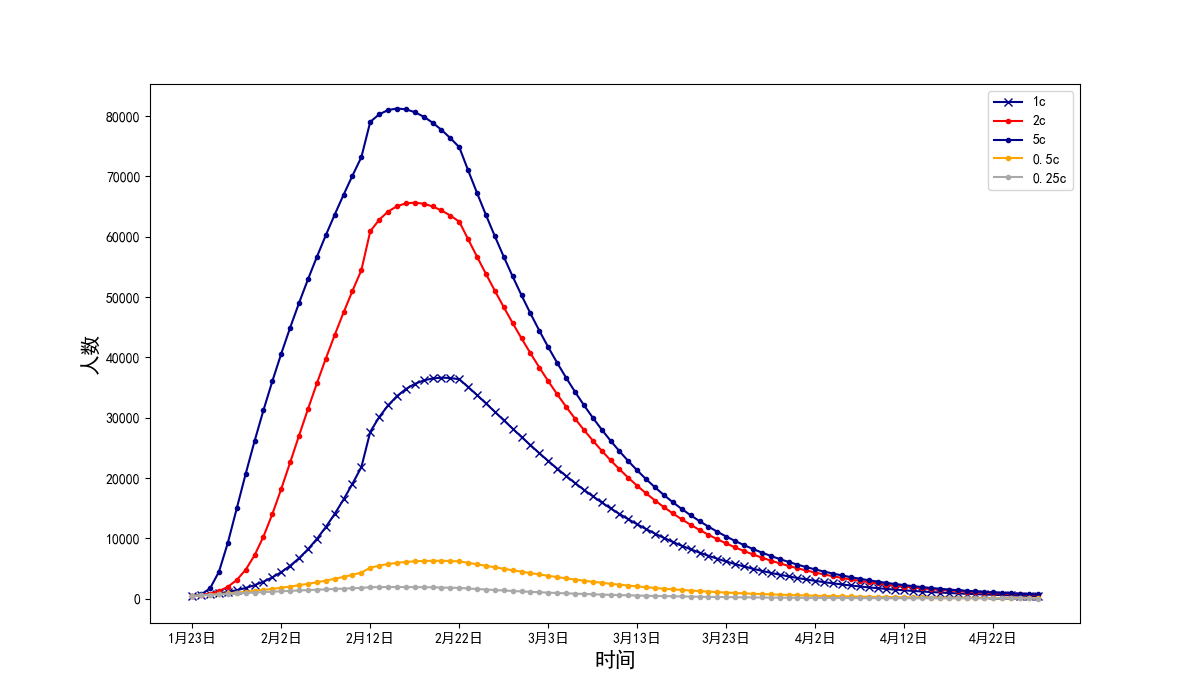
\includegraphics[width=1.0\textwidth]{figures/c.png}
    \caption{不同接触率对疫情传播的影响}
    \label{fig:c}
\end{figure}

分析发现当前疫情防控措施已经对疫情传播产生较好的抑制结果,如果没有武汉封城或延迟采取、市民不自觉居家隔离,武汉市感染人数会迅速增长,并且可能达到当前感染人数2到3倍以上(\cref{fig:c}中蓝色线)。而如果自觉居家隔离、人与人之间交际暂时性大大减少,疫情可以在很短的时间内控制,基本不会造成大规模社会经济损失(\cref{fig:c}中灰色线)。因此,减少人与人的来往、减少接触率是控制疫情传播手段的重中之重。


2020年1月下旬,武汉新建雷神山医院,2月初又建立了20家方舱医院,采取严格的医学追踪隔离,做到应收尽收等措施本质上是增加隔离率,进而减少未被隔离的感染者人数。以原始模型中$q$参数为基点,通过增加隔离率来模拟上述措施提前采取;通过减少隔离率来模拟上述措施没有采取或延迟采取。模拟结果如\cref{fig:h}所示,当隔离比例下降为$0.5q$、$0.25q$时,感染人数的上升速率和峰值均会增加,甚至达到了指数级的上升速率,尤其是隔离比例取$0.25q$时,感染人数峰值提高一倍多。而当隔离比例取$5q$时,感染人数峰值下降了近三倍,感染人数上升相当平缓。由此可见,有效、严格的隔离措施对防止疫情效果颇佳。
\begin{figure}[!h]
    \centering
    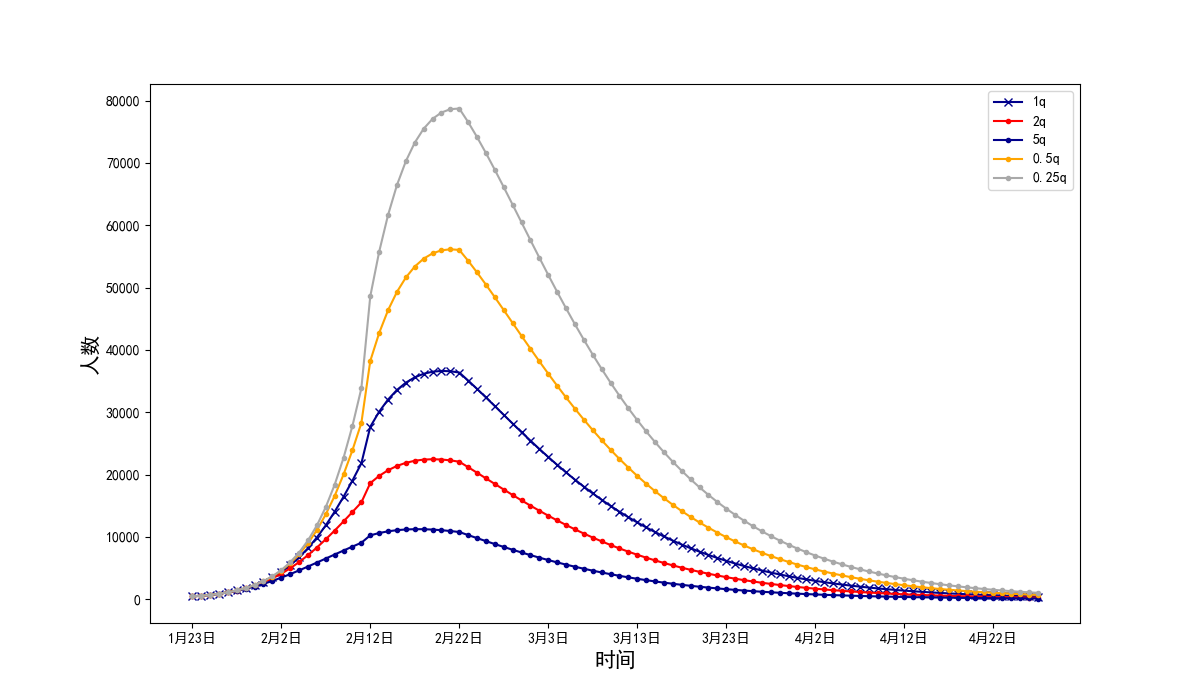
\includegraphics[width=1.0\textwidth]{figures/q.png}
    \caption{不同隔离率对疫情传播的影响}
    \label{fig:h}
\end{figure}


全国各地有近4.2万医务人员驰援武汉抗击疫情,做到应治尽治等措施相当于增加了住院患者治愈率$\gamma_H$,通过减少住院患者治愈率来模拟上述措施未采取或延迟采取;通过增加住院患者治愈率来模拟上述提前采取。\cref{fig:gamma}给出了模拟结果。根据该结果,容易发现是疫情已经爆发的情况下,治愈率的提高是较短时间内控制疫情,使疫情快速结束的直接方法。\cref{fig:gamma}五条线显示,治愈率越高,对疫情扩散、峰值的影响相对隔离率、接触率不是特别大,但对峰值快速下降贡献了重大力量,可以说疫情能够在4月底基本结束得益于治愈率的提高。

\begin{figure}[!h]
    \centering
    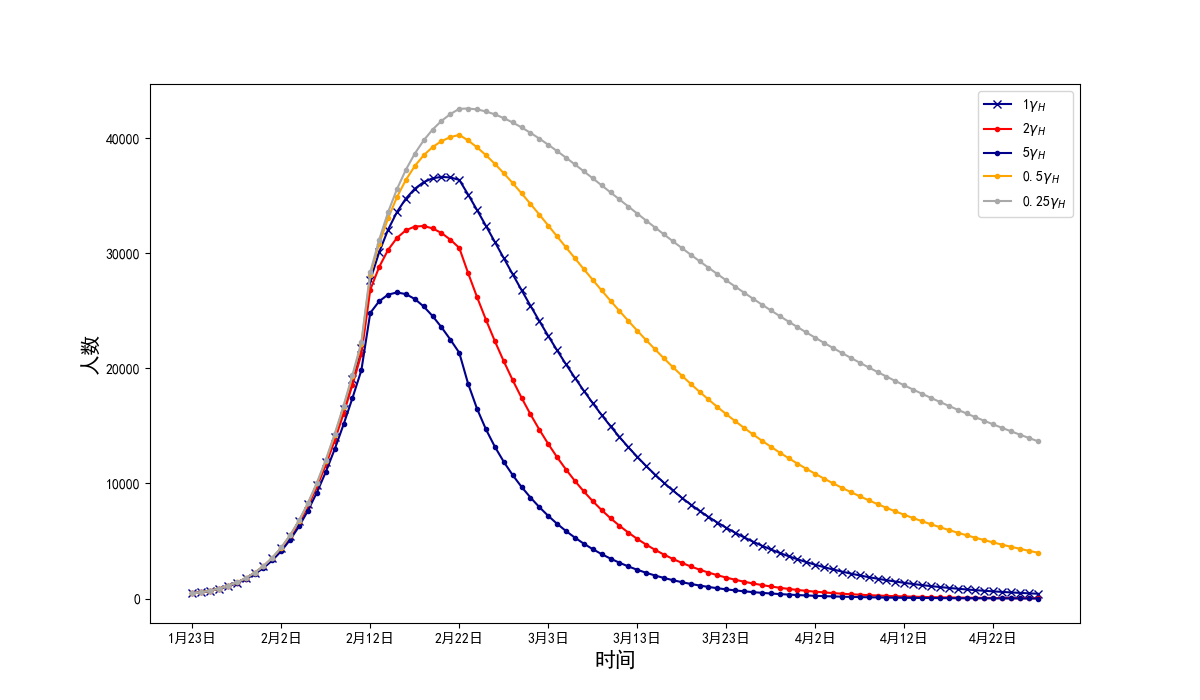
\includegraphics[width=1.0\textwidth]{figures/yh.png}
    \caption{不同治愈率对疫情传播的影响}
    \label{fig:gamma}
\end{figure}



\subsection{问题三}
印度自从2020年1月30日出现第一例确诊,此后表面上并未恶化,直到3 月25 日,印度政府意识到本土疫情的严重性,宣布全国处于封锁状态,当时其累计确诊病例数也只有519 例,死亡病例10 例。印度在5 月30 日宣布放宽部分限制措施,当时印度已经累计报告超过18 万例确诊病例,而且病例数还在增加。当地时间7 月17 日,印度累计报告新冠肺炎确诊病例超过100 万例,
由此成为全球第三个确诊病例数突破100 万例的国家,次于巴西与美国。当
下,印度全国的感染人数仍在以令人担忧的速度飙升。值得一提的是,由于
检测能力有限,印度政府的统计数据无法反映全部情况。


本部分的模型与问题一保持一致。区别在于印度控制措施强度前后无明显变化,因此不再划分时间段,整个时间段采用相同的模型参数,并在参数方面结合印度真实的隔离与治疗情况进行适当调整与修改。

印度疫情初期确诊病例极少,考虑到文献\cite{reference4}“真实的感染病例数,依赖于病毒检测的规模和频率、检测的准确性。很现实的一点就是,印度的检测频率很低。格局印度医学研究理事会(ICMR) 的报告,截至4 月14 日,只有229426 名受试者接受了测试(占总人口的0.03\%).”故该部分模型从疫情有所初势的3月10号开始研究,持续到9月30日,根据3月10号到7月30日的疫情传播情况调整参数,拟合曲线,并预测7月30日至9月30日印度疫情的走向。模型所用参数见\cref{tab:intipara2}、\cref{tab:initvalue2}。结果见\cref{fig:IndiaModel}。

\begin{table}[H]\small
    \caption{问题三:修正SEIR模型参数取值}
    \label{tab:intipara2} \centering
    \begin{tabular}{p{1cm}p{0.7cm}p{0.7cm}p{0.7cm}p{0.7cm}p{0.7cm}p{0.7cm}p{1.5cm}p{0.7cm}p{0.7cm}p{0.7cm}p{0.7cm}}
        \toprule[1.5pt]
        \textbf{变量} & $\beta$ & $\delta_I$ & $\delta_H$ & $\gamma_I$ & $\alpha$ & $\sigma $ & $\lambda$ &$\theta$&$q$&$c$&$\gamma_H$\\
        \midrule[1pt]
        \textbf{取值} & $1.06 \times 10^{-11}$ & 0.7& 0.13& 0.05& $ 2.7 \times 10^{-4} $ & 1/6& 1/14&1&$1.0 \times 10^{-9}$&11.7&0.1\\
        \textbf{取值说明} &  调整&  调整&  \cite{reference1}&  调整&  \cite{reference2}&调整 & 隔离时长为14天& \cite{reference4}& \cite{reference4}& \cite{reference4}&调整\\
        \bottomrule[1.5pt]
    \end{tabular}
\end{table}

\begin{table}[H]\small
    \caption{问题三:修正SEIR模型人群初始值}
    \label{tab:initvalue2} \centering
    \begin{tabular}{p{1.5cm}p{2cm}p{3cm}p{1cm}p{1cm}p{1cm}p{1cm}p{1cm}}
        \toprule[1.5pt]
        \textbf{变量} & $S$ & $E$ & $I$ & $S_q$ & $E_q$ & $H$ & $R$  \\
        \midrule[1pt]
        \textbf{取值} & 1400000000& 55& 5000 &0& 0& 100&3 \\
        \textbf{取值说明} & 估计印度总人口数& 印度3月10日确诊人数与3月17日确诊人数的差值&  估计&  \cite{reference4} &  \cite{reference4}& 估计 &  原数据\\
        \bottomrule[1.5pt]
    \end{tabular}
\end{table}

\begin{figure}[!h]
    \centering
    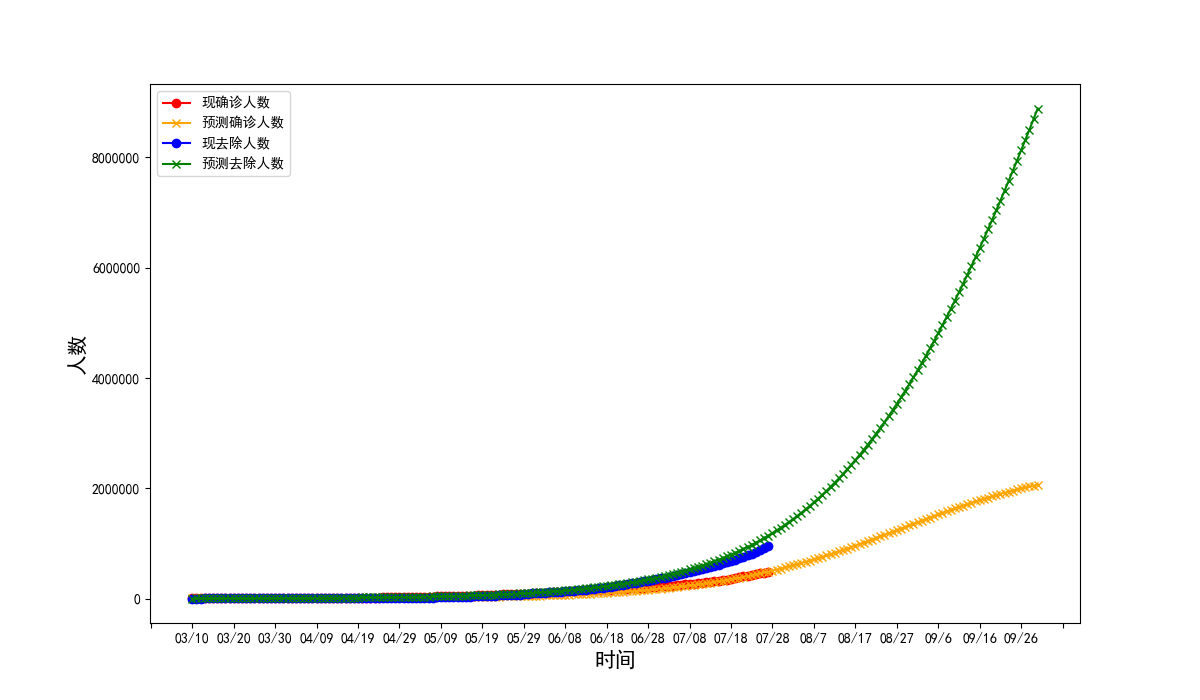
\includegraphics[width=1.0\textwidth]{figures/IndiaModel.png}
    \caption{问题三:印度疫情传播曲线}
    \label{fig:IndiaModel}
\end{figure}

\begin{figure}[!h]
    \centering
    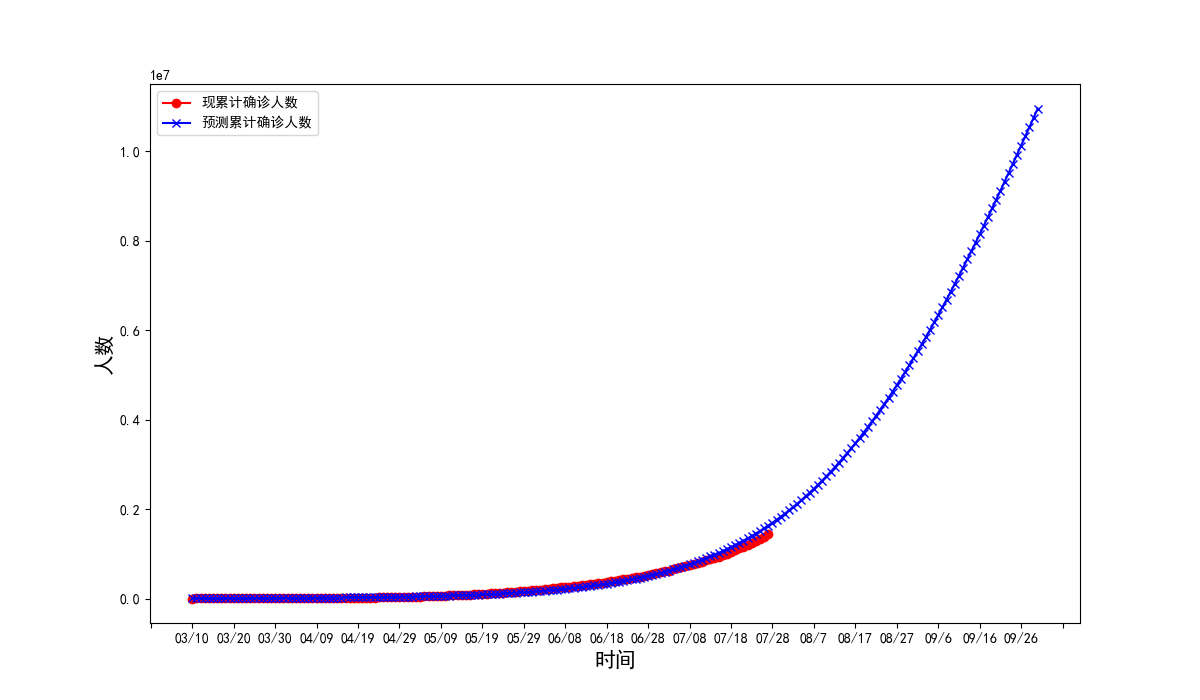
\includegraphics[width=1.0\textwidth]{figures/cumulative.png}
    \caption{问题三:印度疫情累计确诊人数曲线}
    \label{fig:cumulative}
\end{figure}

分析\cref{fig:IndiaModel}发现,模型拟合效果与实际较相符,其中需要注意的是去除人数等于治愈人数+死亡人数。不难发现,实际情况下,去除人数已经比当前确诊人数多了,细细观察原数据集发现印度新冠肺炎治愈率较高。从模型8月到9月底的走势来看,疫情传播丝毫不会式微,还会有大面积的感染,虽然(\cref{fig:IndiaModel}中绿色线)呈指数上升,表明大量感染者能被治愈,但也间接反映仍有非常多正常人被感染,尽管后续会被治愈。更准确反映印度疫情严重性,可见\cref{fig:cumulative},印度累计确诊病例在8月到9月底甚至达到指数级的上升,因此印度政府必须加强疫情防控措施,如严格的追踪隔离、人民提高自我防护意识、减少非需要人与人接触等,否则后果将不堪设想。


\subsection{问题四}

用随机变量$X$表示混样检测中每人检测次数,若$k$人的混合样本呈现阴性,则每人检测次数$X = \frac{1}{k}$,若$k$人的混合样本呈现阳性,则需要对$k$个人单独做检测,每人检测次数$X = 1 + \frac{1}{k}$。因此$X$服从伯努利分布,容易得知:
\begin{equation}
    \left\{\begin{array}{l}
        P\{X=1+\frac{1}{k}\}=1-(1-p)^k \\
        P\{X=\frac{1}{k}\}=(1-p)^k \\
        \end{array}\right.
    \label{equation:1}
\end{equation}
平均每人检测次数,即$X$的数学期望:
\begin{equation}
E(X)=1-(1-p)^k+\frac{1}{k}
\end{equation}

这里的$p$、$k$都是待定的参数,如果经计算得到E(X)<1,那么混样检测方法相比单次检测就能够减轻工作量并降低成本。

本文目的就是在给定$p$值的条件下,使得平均每人检测次数最小。对于混样检测方法,还需考虑$k$值,目标优化表达式即:
\begin{equation}
    \min_{1\leqslant k\leqslant N}  1+(1-p)^k+\frac{1}{k}
    \label{euqation:target}
\end{equation}
其中$k$必须是整数。为方便求导,假设$k$是连续的,对该式做几点数学理论上的分析与解读:\\

\begin{enumerate}
    \item 假设我们已经达到了某个最优点,此时若$p$升高,则与之对应的$k$值不会增大(可能存在不变的情况,因为$k$只能取整数)。这是因为给定一个$p$,达到最优点的一阶条件是
    \begin{equation}
        -\frac{1}{k^2}-\ln(1-p)(1-p)^k=0
    \end{equation}
    而如果将$k$看作$p$的由该方程决定的函数,那么达到极点的条件是
    \begin{equation}
        -\frac{2}{k^3}-(ln(1-p))^2]\frac{dk}{dp}+\frac{1+k(ln(1-p))}{1-p}=0
    \end{equation}
    因为$ln(1-x)<-x,$所以$\displaystyle\frac{1+k(ln(1-p))}{1-p}<\frac{1-kp}{1-p}\leqslant0$,即$\displaystyle\frac{dk}{dp}<0.$
    \item $p$值越高,会导致$E(X)$越高。这是因为:
    \begin{equation}
        \displaystyle\frac{dE(X)}{dp}>0
    \end{equation}          
\end{enumerate}


在给定$p$值条件下,目标函数\label{equation:target}就变成了一个单变量函数最小化问题。
由于$k$是整数,直接求解较有难度。本文先假设$k$为连续值,使用下降单纯形法(Downhill Simplex),近似的求解该目标函数的最小值,以及其对应的最优$k$值。当然,最优的$k$值很大可能是小数,因此还需校准$k$值。本文通过比较$k$值向上取整和向下取整时目标函数大小,来最终确定$k$的最优值。


\cref{fig:k}揭示了最优单组混合样本数量($k$)随病毒携带者比率($p$)变化的条形图。由该图可以看出,随着病毒携带者比率的升高,使其对应目标函数取得最优解的$k$值则随之降低。直观来讲,对于风险较高或者病毒潜在概率较大的地区,混样检测的单组混合样本数量应该较少,这样才能最大程度地节约成本、减少总的检测次数。
\begin{figure}[!h]
    \centering
    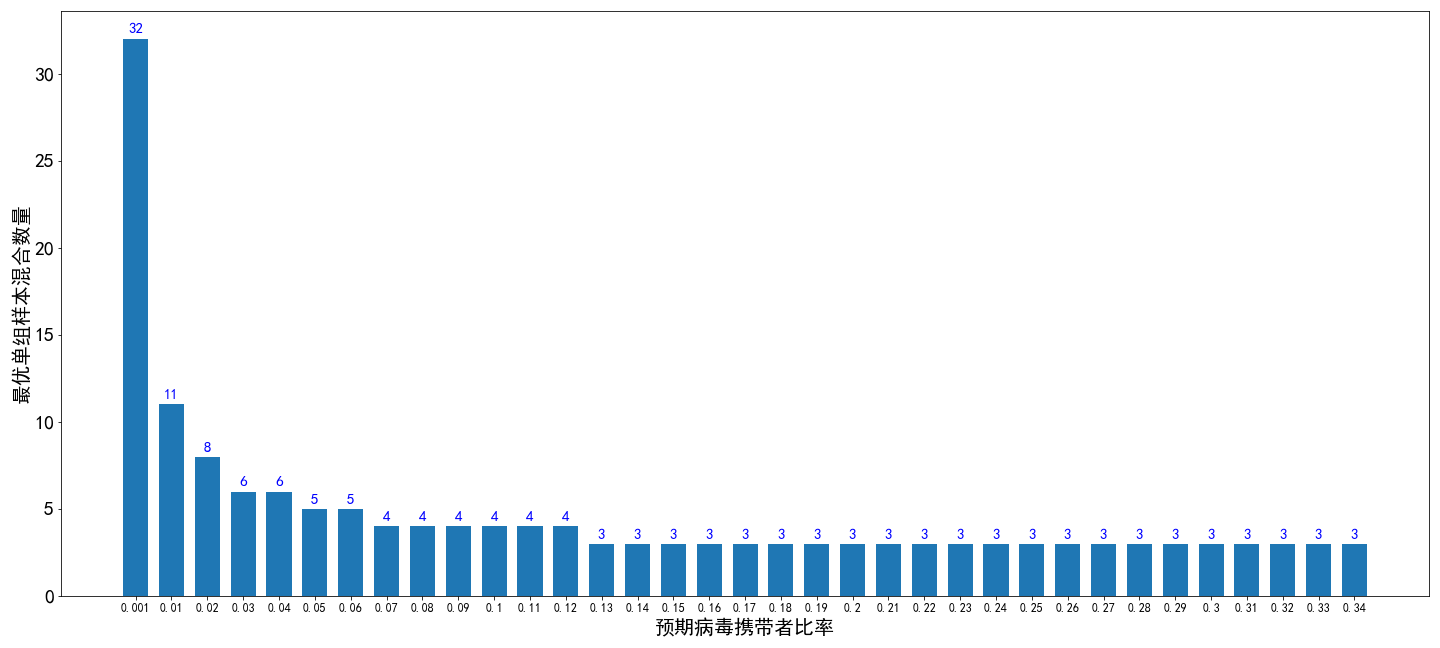
\includegraphics[width=1.0\textwidth]{figures/optimize_pool_size.png}
    \caption{最优$k$值随$p$值的分布}
    \label{fig:k}
\end{figure}


\cref{fig:average}揭示了在每一个给定的$p$值变化条件下,目标函数所能取得的最优值,也即单人需做核酸检测次数期望值E(X)的最小值。从图中可以看出,随着病毒携带者比率的升高,单人所需做的核酸检测数也逐渐升高,这也符合直观。特别地,由图中可以看出,当$p$值达到0.3左右时,E(X)已经接近1,这说明,当人群中病毒携带者比率超过30\%时,应该采用单次检测而非混养检测的方法。

\begin{figure}[!h]
    \centering
    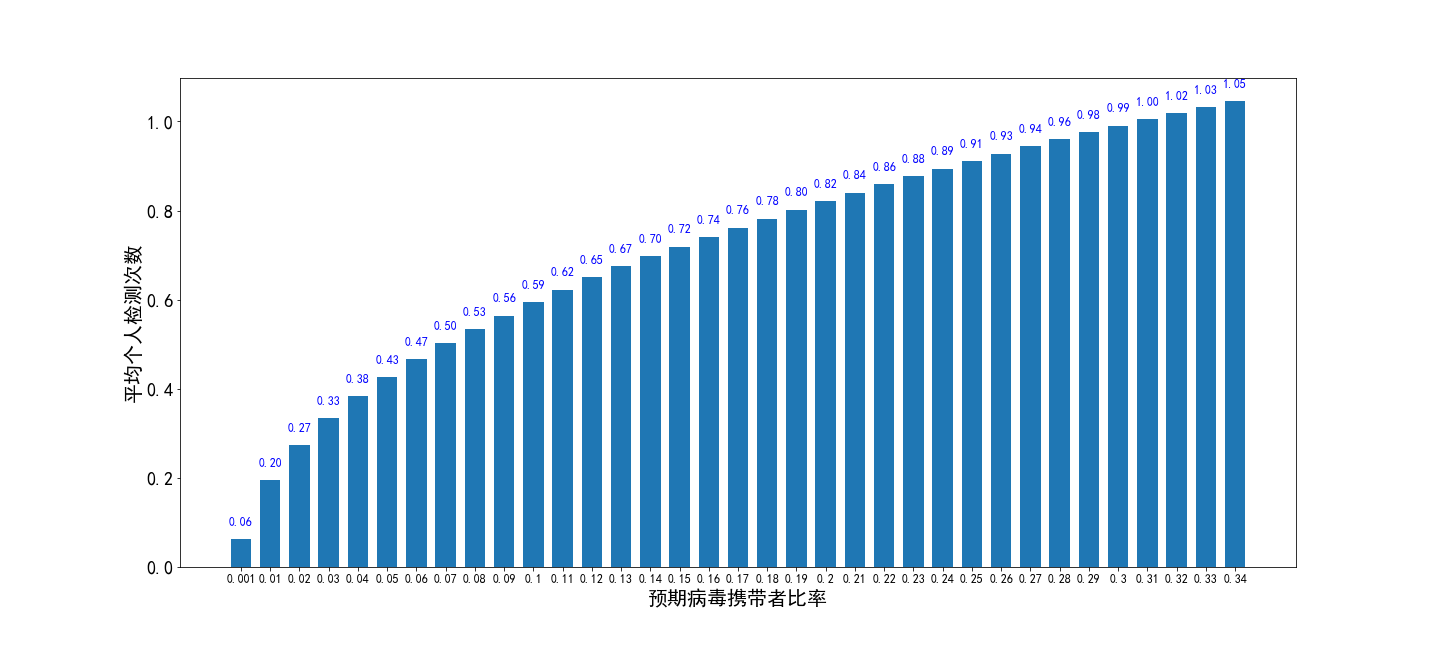
\includegraphics[width=1.0\textwidth]{figures/average_detect.png}
    \caption{平均每人检测次数随$p$值的分布}
    \label{fig:average}
\end{figure}

再来讨论武汉实际核酸检测问题。武汉人口约1108100人,最终确诊人数8万多人,考虑到无症状感染者未计算在内,武汉地区实际感染率约为0.01,即$p=0.01$。根据\cref{fig:k},\cref{fig:average}的结果,在本文模型中,武汉平均每人检测次数为0.20,相当于节约了80\%的成本,混合样本容量以11为宜,这与实际武汉市将10个人的样本混合检测基本相符。


\section{模型评价与改进}
\subsection{模型的优点}
\begin{enumerate}
    \item 问题一、问题二、问题三利用修正的SEIR模型建立新冠疫情传播模型,相比经典的SEIR模型,考虑到了隔离易感者、隔离潜伏者、住院患者,与实际防疫措施贴切。在武汉、印度实际数据上均获得了很好的拟合效果。
    \item 修正的SEIR模型通过改变参数,可以对防疫措施进行评估,指导未来的疫情防控工作。
    \item 问题四利用伯努利分布及下降单纯形法,准确计算了混合检测方法的平均每人检测次数,与单次检测作比较,合理得出了给定人群病毒携带率的有效方案。
\end{enumerate}
\subsection{模型的缺点}
\begin{enumerate}
    \item 修正的SEIR模型没有考虑无症状感染者。
    \item 修正的SEIR模型参数过多,调参任务繁琐。
\end{enumerate}


%参考文献
\begin{thebibliography}{9}%宽度9

    \bibitem[1]{reference1}
    Xia W, Sanyi T, Yong C, et al.
    \newblock  When will be the resumption of work in Wuhan and its surrounding areas during COVID-19 epidemic? A data-driven network modeling analysis[J]. SCIENTIA SINICA Mathematica, 2020.

    \bibitem[2]{reference2}
    曹盛力, 冯沛华, 时朋朋. 
    \newblock 修正 SEIR 传染病动力学模型应用于湖北省 2019 冠状病毒病 (COVID-19) 疫情预测和评估[J]. 浙江大学学报 (医学版), 2020, 49(1): 0-0.

    \bibitem[3]{reference3}
    Lakdawalla D, Keeler E, Goldman D, et al. 
    \newblock Getting Americans back to work (and school) with pooled testing[J]. USC Schaeffer Center White Paper, 2020.
    
    \bibitem[4]{reference4}
    Sarkar K, Khajanchi S, Nieto J J. 
    \newblock Modeling and forecasting the COVID-19 pandemic in India[J]. Chaos, Solitons \& Fractals, 2020: 110049.

\end{thebibliography}

\end{document} 